\documentclass[bsc,singlespacing,logo, parskip, deptreport]{infthesis}

\usepackage{amsmath}
\usepackage{amsfonts}
\usepackage{bm}
\usepackage{url}
\usepackage{hyperref}
\usepackage{tikz}
\usetikzlibrary{bayesnet}

\begin{document}

\title{Automatic Harmonic Analysis of Melodies}

\author{Finlay McAfee}

\course{Master of Informatics}
\project{{\bf MInf Project (Part 2) Report}}

\date{\today}

\abstract{
}

\maketitle
%\includeshield
\begin{acknowledgements}
I would like to thank Mark Steedman and Andrew McLeod for their advice and guidance on this project.
\end{acknowledgements}
\standarddeclaration
\tableofcontents

%\pagenumbering{arabic}

%Summarize contributions
\chapter{Introduction}
This is a report to detail the work carried out in the second year of the MInf Project.

\section{Summary of contributions}

\section{Previous Year}


%Summarize knowledge needed to understand project
\chapter{Theoretical Background}
This chapter goes through the main concepts necessary to understand the design of the systems built in this project. Each section is intended to provide a brief summary of the necessary information on each topic to allow the reader to fully understand the workings of the models in the next chapter, as well as an understanding of the design choices.

\section{Music Theory}
It is safely assumed that the reader is familiar with the concept of music. If not then it is suggested that they study the following albums before returning to read this report: Blood On The Tracks by Bob Dylan \cite{dylan1975blood} and Songs From a Room by Leonard Cohen \cite{cohen2007songs}.

Music is fundamentally concerned with two concepts: rhythm and pitch. Rhythm is, at its simplest, a regularly repeating pattern. The periods of repetition that musical rhythm is most concerned with lie around the same frequency as that of the human gait, or heart beat (the reader is left to draw their own conclusions about the significance of this). Pitch is, essentially, also concerned with regularly repeating patterns, only now the domain is hundreds of beats per second. The human ear experiences this as a musical note, rising and falling in pitch as the frequencies increase and decrease.

Music has been studied and practised by many different cultures over the course of human history and there have been many different formalisms for describing it developed. The most common, and that used in this report is {\em Western Tonal Music} (WTM). Under this paradigm, the continuous range of pitch is divided into repeating {\em octaves}, where corresponding points on each {\em octave} are perceived as the same note at different pitches. These ranges are then subdivided into 12 distinct notes. The method used for these divisions is based on ratios between note frequencies, the most commonly used being Equal Temperament \cite{regener1973pitch}. Pieces of music are organised into one of 12 {\em keys}, each with a {\em tonic} corresponding to one of the 12 notes. Keys can be thought of as a prior over the distribution of notes in a song, where the tonic note has the highest probability of being played.

In written music, pitch is associated with vertical direction on a {\em stave}, shown below.

DIAGRAM.

Rhythm is concerned with the temporal positioning of these notes, both where and when they occur, as well as for how long to play them. In WTM a piece of music has an associated beat or {\em tempo} that defines the frequency of an underlying, unheard pulse, over which the notes of the piece are laid, typically close to 120 beats per minute. The {\em time signature} of a piece defines how to treat groups of these beats, with the most common being $\frac{4}{4}$. This corresponds to groupings of four beats (also called {\em quarter notes} or {\em crotchets}). These groupings are referred to as {\em bars} and are used to organise the temporal structure of a melody in a way that is both easy to read and represents the underlying rhythmic properties of the piece. As in western languages, time flows from left to right in written music.

DIAGRAM

The above is a very brief overview of melodic structure in a piece of music. However there is another concept that is fundamental to this problem space, and that is {\em harmony}. Fundamentally, {\em harmony} is the relationship between the pitches of two notes, as they are heard together. It is concerned with the {\em intervals} between the notes and how they are perceived. The most basic interval is the {\em semitone}, the distance between one note and its neighbour, hence there are 12 semitones in an octave. The harmonic perception of an interval of two or less semitones is dissonant and jarring. The octave itself is an interval, which is perceived as resonant and uncharacterised, another way of saying that two pitches an octave apart are perceived as the same note. The next simplest interval is when two notes are 5 semitones apart, the {\em perfect fifth}, referred to as a {\em power chord} in guitar terminology, it adds the most basic harmonic colour. The intervals of 3 and 4 semitones are where harmony takes on an emotional quality, 3 semitones is referred to as a {\em minor third}, and evokes a feeling of darkness and melancholy, when perceived; whereas 4 semitones, the {\em major third} evokes the opposite emotion, that of brightness. It is this incredible connection between emotions and intervals that makes musical harmony so fascinating.

INTERVAL DIAGRAM

A {\em chord} is when more than one note is played at one point in time, typically at least three. The basic three-note chord is called a {\em triad}, composed of notes that are based on intervals, relative to the note in the first position, the {\em root}. The other two are the {\em perfect fifth} and a {\em third}, either {\em major} or {\em minor}. Depending on the {\em third} that is chosen, the full chord with take on one of these qualities. The following diagram shows the basic C major chord.

DIAGRAM OF C CHORD

A modern musical arrangement, for example a jazz standard, typically consists of both a melody and an associated progression of chords, intended to be played as an accompaniment to the melody. The problem space of this project is concerned with the association between these two, specifically the problem of generating one if the other is not present. Generating a melody is what is typically considered musical composition, a difficult problem to solve on which much work has been done in recent years CITE ALL THE THINGS. This project concerns itself with the other direction, predicting chord sequences from melodies. This problem is conceptually half sequential classification, half generation, as there is not necessarily a unique chord sequence for every melody, but there is still a ground truth that can, theoretically, be derived from the observed notes. The following piece of music is an example from one of the corpora used for training the models.

DIAGRAM MINUET IN G

DISCUSS WITH WORKED EXAMPLE ON ABOVE

In terms of a traditional classification problem, $f(x) = y$, the $x$ here is a sequence of notes and the $y$ is a sequence of chord labels. Hence we have a sequence to sequence problem.

\section{Inspiration from Natural Language Processing}

An often-drawn comparison is that of the similarity between music and language. Many postulate that music is itself a form of language \cite{cohen2008music} (although perhaps it is more enlightening to say that language is a music). This is useful when analysing music as there is a wealth of literature on natural language processing.

The immediate comparison that can be drawn is to Part of Speech (POS) Tagging. In this problem we are trying to assign grammatical tags to a tokenized sequence of words, for example:

And/CC now/RB for/IN something/NN completely/RB different/JJ

This one-to-one mapping problem is analogous to chord labelling in the case where each note is labelled with a corresponding chord:

c/Cmaj d/Cmaj e/Emin f/Emin g/Gmaj

We can describe this in terms of latent variables $h_i$ and visible variables $v_i$:

\begin{center}
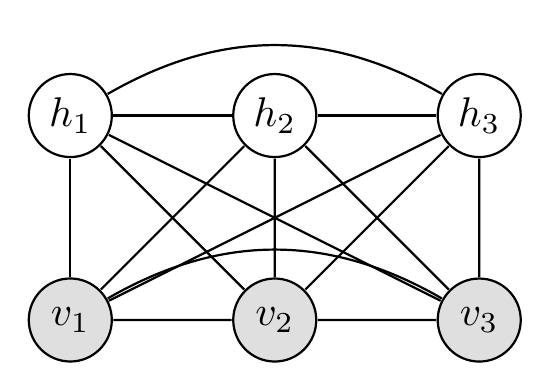
\begin{tikzpicture}[thick,scale=1.5, every node/.style={transform shape}]
  % Nodes
  \node[latent]       (h1)        {$h_1$};
  \node[latent, right = of h1]       (h2)        {$h_2$};
  \node[latent, right = of h2]       (h3)        {$h_3$};
  \node[obs, below = of h1]       (v1)        {$v_1$};
  \node[obs, right = of v1]       (v2)        {$v_2$};
  \node[obs, right = of v2]       (v3)        {$v_3$};
  % Connections
  \draw[] (h1) -- (h2);
  \draw[] (h2) -- (h3);
  \path[] (h1) edge [bend left] (h3);
  \draw[] (v1) -- (v2);
  \draw[] (v2) -- (v3);
  \path[] (v1) edge [bend left] (v3);
  \draw[] (h1) -- (v1);
  \draw[] (h2) -- (v2);
  \draw[] (h3) -- (v3);
  \draw[] (h1) -- (v2);
  \draw[] (h1) -- (v3);
  \draw[] (h2) -- (v1);
  \draw[] (h3) -- (v1);
  \draw[] (h2) -- (v3);
  \draw[] (h3) -- (v2);
\end{tikzpicture}
\end{center}

Both are examples of a problem where the visible variables that are observed are dependant on the latent variables that are trying to be determined. As can be seen in the diagram above, the naive approach introduces a large number of connections to model.  This problem would be simpler if said latent and observed variables were not dependant on each other, and each observed variable only depended on one hidden variable:

\begin{center}
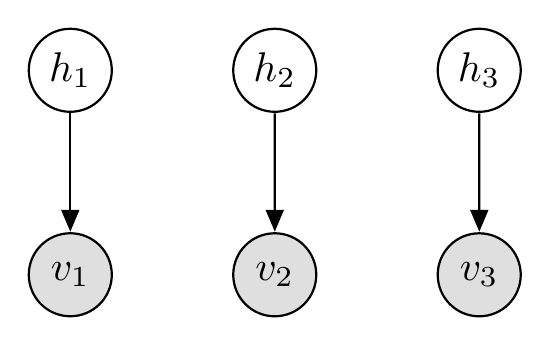
\begin{tikzpicture}[thick,scale=1.5, every node/.style={transform shape}]
  % Nodes
  \node[latent]       (h1)        {$h_1$};
  \node[latent, right = of h1]       (h2)        {$h_2$};
  \node[latent, right = of h2]       (h3)        {$h_3$};
  \node[obs, below = of h1]       (v1)        {$v_1$};
  \node[obs, right = of v1]       (v2)        {$v_2$};
  \node[obs, right = of v2]       (v3)        {$v_3$};
  % Connections
  \edge[] {h1} {v1};
  \edge[] {h2} {v2};
  \edge[] {h3} {v3};
\end{tikzpicture}
\end{center}

But this is clearly not the case. An adjective is very likely to be followed by a noun, and a G major is very likely to be followed by a C major. In reality the situation looks more like this:

\begin{center}
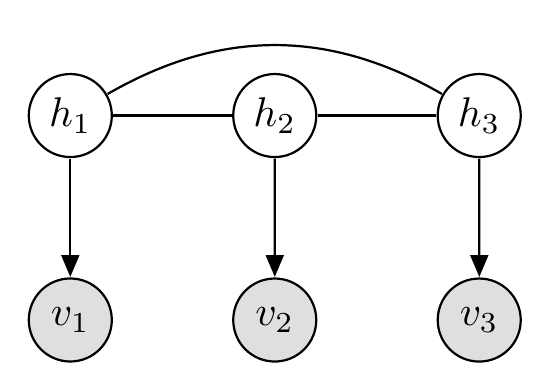
\begin{tikzpicture}[thick,scale=1.5, every node/.style={transform shape}]
  % Nodes
  \node[latent]       (h1)        {$h_1$};
  \node[latent, right = of h1]       (h2)        {$h_2$};
  \node[latent, right = of h2]       (h3)        {$h_3$};
  \node[obs, below = of h1]       (v1)        {$v_1$};
  \node[obs, right = of v1]       (v2)        {$v_2$};
  \node[obs, right = of v2]       (v3)        {$v_3$};
  % Connections
  \draw[] (h1) -- (h2);
  \draw[] (h2) -- (h3);
  \path[] (h1) edge [bend left] (h3);
  \edge[] {h1} {v1};
  \edge[] {h2} {v2};
  \edge[] {h3} {v3};
\end{tikzpicture}
\end{center}

It is useful to assume independence of observed variables given the latent variables and this is something that all the models do, but the relationship between the $h_i$ are more complex and this is one area where the difficulty arises in these problems. An often used approach to this is to apply the first-order Markov Assumption. This allows us to assume that each latent variable $h_t$ is only dependant on the previous latent variable $h_{t-1}$ in a temporal ordering $t \in \{1:T\}$. This model is known as a Hidden Markov Model (HMM). POS Tagging is a success story for the HMM \cite{kupiec1992robust}. 

\begin{center}
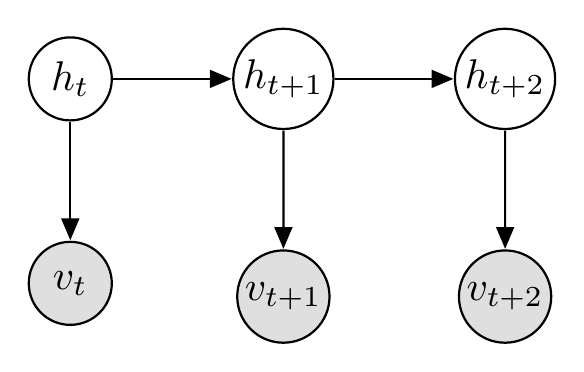
\begin{tikzpicture}[thick,scale=1.5, every node/.style={transform shape}]
  % Nodes
  \node[latent]       (h1)        {$h_t$};
  \node[latent, right = of h1]       (h2)        {$h_{t+1}$};
  \node[latent, right = of h2]       (h3)        {$h_{t+2}$};
  \node[obs, below = of h1]       (v1)        {$v_t$};
  \node[obs, below = of h2]       (v2)        {$v_{t+1}$};
  \node[obs, below = of h3]       (v3)        {$v_{t+2}$};
  % Connections
  \edge[] {h1} {h2};
  \edge[] {h2} {h3};
  \edge[] {h1} {v1};
  \edge[] {h2} {v2};
  \edge[] {h3} {v3};
\end{tikzpicture}
\end{center}

\section{Hidden Markov Models}

The HMM assumes an underlying latent state space $\mathcal H$, with transition probabilities between members. These variables are conditionally independent of each other, given the previous $h_{t-1}$, i.e. the first-order Markov Assumption:

\begin{align}
  P(h_t | h_{t-1}),& \quad h_t, h_{t-1} \in {\mathcal H}, \quad  t \in \{1:T\} \\
  I(h_t, h_i | h_{t-1}),&  \quad i \in \{1:T\}
\end{align}

And a visible variable space $\mathcal V$, which are conditionally independent of each other given the corresponding latent variable at time $t$:

\begin{align}
  P(v_t | h_t),& \quad h_t \in {\mathcal H}, \quad v_t \in {\mathcal V}, \quad  t \in \{1:T\} \\
  I(v_t, v_i | h_{t}),& \quad \forall i \in \{1:T\}
\end{align}

Given these assumptions we can write the entire joint probability distribution as:

\begin{equation}
  P(\{v_{t}\}^{T}_{t=1}, \{h_{t}\}^{T}_{t=1}) = P(v_1 | h_1) P(h_1) \prod_{t=2}^{T} P(v_t | h_t) P(h_t | h_{t-1})
\end{equation}

Which simplifies the complexity of the problem enormously.

There are various forms of inference that can be performed on HMMs. In the case of on-line accompaniment prediction, the probability we are interested in would be $P(h_{t+1} | \{v_i\}_{i=1}^{t})$. This can be performed by first summing over all possible states at time $t$, then calculating probabilities of those $h_t$ by propagating recursively back to the start state. This is referred to as the forward algorithm or {\em filtering} \cite{russell2002artificial}. In terms of message passing in graphical inference, the message is being passed from all observed variables $\{v_i\}_{i=1}^{t}$, starting at $t=1$, summing over the latent variables $h_t$ as the message is passed up the chain.

The case looked at for this report is concerned with the off-line variant of this problem, predicting the most probable sequence of latent variables, given the full observed sequence:

\begin{equation}
  {\mathrm arg}\max_{\{h\}_{t=1}^{T}} P(\{h\}_{t=1}^{T} | \{v\}_{t=1}^{T})
\end{equation}

This is calculated by a form of dynamic programming called the Viterbi Algorithm \cite{russell2002artificial}, see section \ref{HMM IMP}.

So this model allows us to generate the most likely sequence of hidden, latent variables given an observed sequence, with the assumptions the each observed variable is only dependant on the others {\em through} its corresponding latent variable, and that each latent variable is only dependant on its past {\em through} the previous time step, and is entirely independent of its future. See section \ref{HMM DES} for a discussion on the problems these assumptions raise for this problem space.

\section{Neural Networks}

One immediate concern with the HMM is that it is unable to capture long term dependencies. It is memoryless, or, more accurately, can only remember one thing: the last place it visited. This contradicts our intuitive grammatical understanding of language. A grammar is a tree structured language model, where the following section can be very dependant on something that happened at the start of the sequence. One example of this in music is repeated phrases; you can't repeat something if you have forgotten it.

What we want is a model that can carry information through it then learn when to forget it and when to incorporate it into deciding the output at a given time. A popular model for this type of system is the Recurrent Neural Network (RNN), in particular with a Long Short Term Memory (LSTM) cell.

Work on neural networks architectures has flourished in the past few years, due largely in part to advances in optimised computation on GPUs \cite{oh2004gpu}\cite{krizhevsky2012imagenet}, as well as new pre-training methods such as autoencoders \cite{hinton2006reducing}\cite{vincent2008extracting}\cite{deng2010binary}. However the basic concept has not changed very significantly since its their beginnings in Hebbian Learning and the Perceptron in the 1940s and 1950s \cite{hebb1949first} \cite{rosenblatt1958perceptron}.

\subsection{Perceptrons and MLPs}

A perceptron is a linear classifier based on an abstraction of a neuron. It is, in essence, a weighted sum of inputs with one output.

\begin{center}
  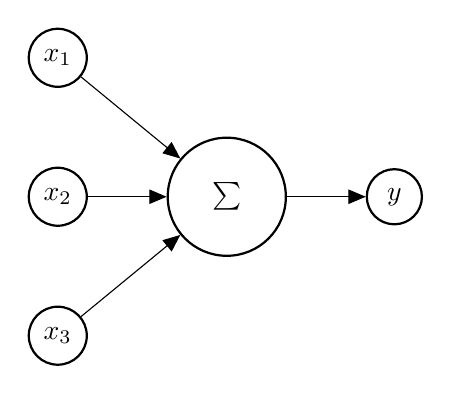
\begin{tikzpicture}[perceptron/.style={circle, draw, thick, minimum size=15mm}, input/.style={circle, draw, thick, minimum size=7mm}]
    % Nodes
    \node[perceptron] (p)   {$\sum$};
    \node[input, left = of p]      (x2)  {$x_2$};
    \node[input, above = of x2]      (x1)  {$x_1$};
    \node[input, below = of x2]      (x3)  {$x_3$};
    \node[input, right = of p] (out) {$y$};
    % Connections
    \edge[] {x1} {p};
    \edge[] {x2} {p};
    \edge[] {x3} {p};
    \edge[] {p} {out};
  \end{tikzpicture}
\end{center}

The key observation is that these weights can be trained to create a binary classification model, where the two classes are linearly separable. The classic example of a problem this model cannot solve is the XOR logic gate, as in this case a straight line cannot be drawn which separates the two classes \cite{minsky1969perceptrons}.

If we take a row of perceptrons with the same inputs but different weights, we now have one layer of a Multi Layer Perceptron (MLP). MLPs are built by taking the outputs of these layers, applying an activation function such as a logistic sigmoid ($\sigma$) or a hyperbolic tangent ($tanh$), then treating these values as the inputs to another layer.

\begin{center}
  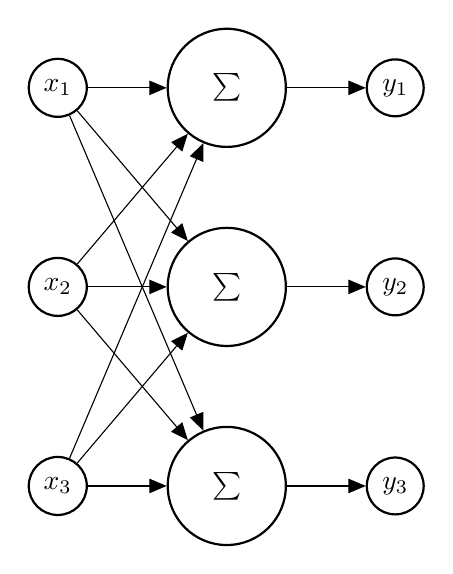
\begin{tikzpicture}[perceptron/.style={circle, draw, thick, minimum size=15mm}, input/.style={circle, draw, thick, minimum size=7mm}]
    % Nodes
    \node[perceptron] (p2)   {$\sum$};
    \node[perceptron, above = of p2] (p1)   {$\sum$};
    \node[perceptron, below = of p2] (p3)   {$\sum$};
    \node[input, left = of p2]      (x2)  {$x_2$};
    \node[input, left = of p1]      (x1)  {$x_1$};
    \node[input, left = of p3]      (x3)  {$x_3$};
    \node[input, right = of p2] (out2) {$y_2$};
    \node[input, right = of p1] (out1) {$y_1$};
    \node[input, right = of p3] (out3) {$y_3$};
    % Connections
    \edge[] {x1} {p1};
    \edge[] {x2} {p1};
    \edge[] {x3} {p1};
    \edge[] {x1} {p2};
    \edge[] {x2} {p2};
    \edge[] {x3} {p2};
    \edge[] {x1} {p3};
    \edge[] {x2} {p3};
    \edge[] {x3} {p3};
    \edge[] {p1} {out1};
    \edge[] {p2} {out2};
    \edge[] {p3} {out3};
  \end{tikzpicture}
\end{center}

Another name for these models are Feed-Forward Artificial Neural Networks (ANNs). By continuing like this we can build an arbitrarily large ANN, which can be used to model more and more complex problems. In fact it can be proven that even just a single layer, finite length ANN can be used to approximate any continuous function on compact subsets of ${\mathbb R}^n$ \cite{cybenko1989approximation}\cite{hornik1989multilayer}. This astounding property, known as the Universal Approximation Theorem, is one of the reasons that neural networks are outperforming many traditional mathematical models currently, in a variety of fields from computer vision \cite{krizhevsky2012imagenet} to protein modelling \cite{uziela2017proq3d}.

However this theorem gives no algorithm for building these complex models. The difficulty comes in training the weights to correctly model the problem, and in the cases of very deep models this can mean millions of parameters. Even worse, there is no analytic solution in optimising these parameters, they must be trained iteratively. This means a large amount of computation time and resources.

To train an ANN in a supervised manner, an error function is needed between the output of the network and the training labels. To continue the notation introduced in the HMM section we will let the $\{v_i\}_{i=1}^{T}$ be the input to the network, $\bm{v}$ using vector notation. The output variables are re-named $\{y_i\}_{i=1}^{S}$, or $\bm{y}$, to avoid confusion with the hidden layers of the network, $\bm{h}_i$, for the $i$th layer. Let the training label associated with $\bm{y}$ be denoted $\bm{t}$. A superscript in parentheses, $\bm{y}^{(j)}$, will be used to denote the $j$th instance of data, from a data sample of size $N$. In the case of three layers, this will look like:

\begin{center}
  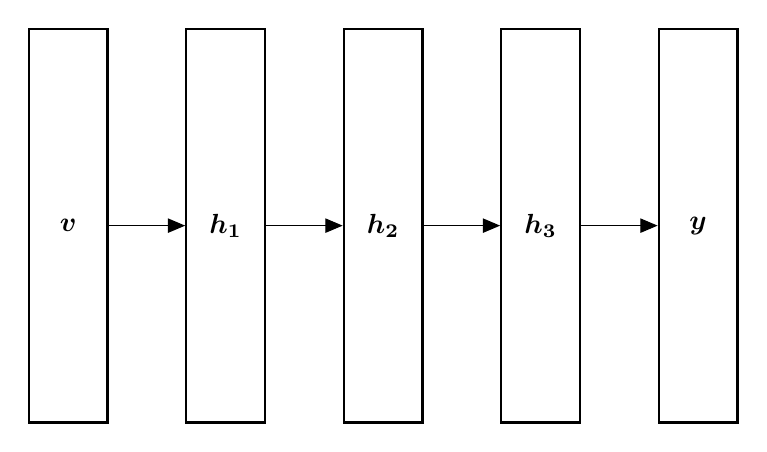
\begin{tikzpicture}
    % Layers
    \node [draw,thick,minimum width=1cm,minimum height=5cm] (v) {$\bm{v}$};
    \node [right of = v, draw,thick,minimum width=1cm,minimum height=5cm, node distance = 2cm] (h) {$\bm{h_1}$};
    \node [right of = h, draw,thick,minimum width=1cm,minimum height=5cm, node distance = 2cm] (h2) {$\bm{h_2}$};
    \node [right of = h2, draw,thick,minimum width=1cm,minimum height=5cm, node distance = 2cm] (h3) {$\bm{h_3}$};
    \node [right of = h3, draw,thick,minimum width=1cm,minimum height=5cm, node distance = 2cm] (y) {$\bm{y}$};
    % Connections
    \edge {v} {h}
    \edge {h} {h2}
    \edge {h2} {h3}
    \edge {h3} {y}
  \end{tikzpicture}
\end{center}

Hence we have an error function:

\begin{equation}
  \label{error}
  \sum_{j = 1}^{N} E(\bm{y}^{(j)}, \bm{t}^{(j)})
\end{equation}

The weights are then updated in a way that minimises this error function. To do this it is necessary to take the derivative of the error with respect to each weight. This is simple to do with a single layer but becomes more complex with a deep network. The method for achieving this is called Back Propagation and was created by Paul Werbos in 1974 \cite{werbos_1974}. Methods for iteratively updating the gradients based on these derivatives are called Gradient Descent and tend to take the following form:

\begin{equation}
  w_{ik} := w_{ik} - \eta \frac{\partial E(\bm{y}, \bm{t})}{\partial w_{ik}}
\end{equation}

Where $w_{ik}$ is the $k$th weight of the $i$th layer. These gradients can either be done per data point $j$ or by summing over batches as in \ref{error}. By this method the neural network can be slowly pivoted towards on optimal configuration, but there is no guarantee of avoiding local minima, and even if it manages to perfectly fit the training data, it will likely be overfit and not generalise to held out test data. Despite these problems, advances in processing speeds and hardware level algorithms \cite{kruger2003linear} have made training these models possible.

\subsection{Recurrent Neural Networks and LSTMs}

So is it possible to use neural networks to predict a sequence of chords from a sequence of notes? Unfortunately, in the current state described, the ANN takes a vector $\bm{v}$ of fixed-size $T$ as input, and outputs $\bm{y}$ of fixed size $S$. What is needed is a network with a flexible input and output size, a tricky problem under the current architecture as this would been adding and removing weights for every data sample. Recurrent Neural Networks (RNNs) solve exactly this problem.

An RNN is a neural network that scales dynamically to it's input. It is composed of {\em cells} that share weights and are connected together in a chain. A single RNN cell looks like a standard feed-forward network, but it's input $v_t$ is combined with an output from the previous cell $h_{t-1}$. Architectures vary but it is common for the output of the cell, $y_t$, to be the output of a second layer that takes $h_t$ as input, and for the output of this hidden layer, $h_t$, to be passed to the next cell in the chain. Of course these cells can be further stacked to result in deeper architectures that learn higher-level features of their input.

The following diagram represents a simple, one-layer RNN, where the full layers are now represented as circular nodes, for compactness and comparison to the HMMs (note in the HMMs the arrows represent dependence relationships, here they represent weighted sums and activations, but the concept is similar):

\begin{center}
  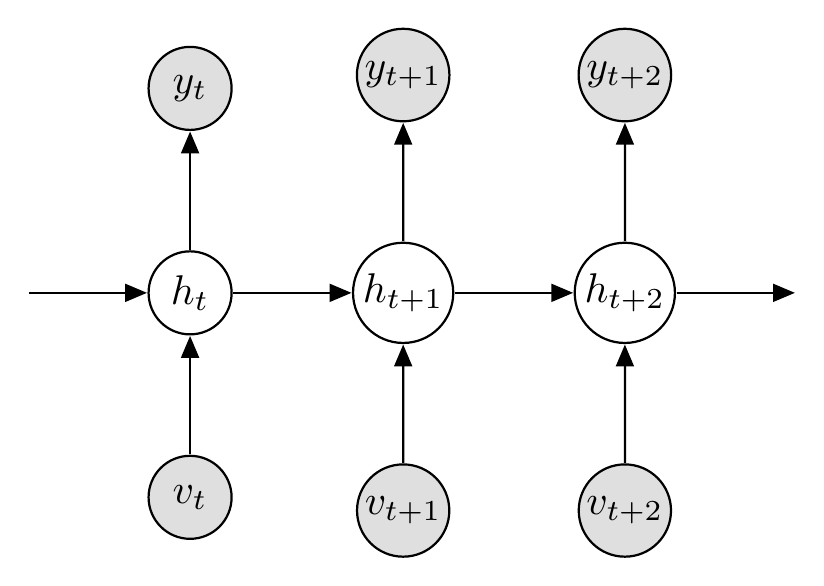
\begin{tikzpicture}[thick,scale=1.5, every node/.style={transform shape}]
  % Nodes
  \node[latent]       (h1)        {$h_t$};
  \node[latent, right = of h1]       (h2)        {$h_{t+1}$};
  \node[latent, right = of h2]       (h3)        {$h_{t+2}$};
  \node[obs, below = of h1]       (v1)        {$v_t$};
  \node[obs, below = of h2]       (v2)        {$v_{t+1}$};
  \node[obs, below = of h3]       (v3)        {$v_{t+2}$};
  \node[obs, above = of h1]       (y1)        {$y_t$};
  \node[obs, above = of h2]       (y2)        {$y_{t+1}$};
  \node[obs, above = of h3]       (y3)        {$y_{t+2}$};
  \coordinate[left = of h1] (hneg);
  \coordinate[right = of h3] (hpos);
  % Connections
  \edge[] {hneg} {h1}
  \edge[] {h3} {hpos}
  \edge[] {h1} {h2};
  \edge[] {h2} {h3};
  \edge[] {v1} {h1};
  \edge[] {v2} {h2};
  \edge[] {v3} {h3};
  \edge[] {h1} {y1};
  \edge[] {h2} {y2};
  \edge[] {h3} {y3};
\end{tikzpicture}
\end{center}

To train these models we can unfold them after receiving all of the input, so that it looks like a complex feed-forward model, that back propagate the error in a similar method to before, now called Back Propagation Through Time (BPTT) \cite{werbos1990backpropagation}.

A problem with this method, referred to as the vanishing gradient problem \cite{hochreiter1998vanishing}, is where the earlier weights in the network receive a much smaller update than those closer to the final output, as the back propagated gradient at time $t$ has been through $T - t$ applications of the chain rule, each involving multiplication with numbers $< 1$, resulting in the gradient becoming incredibly small. Hence errors caused by weights near the start of the sequence won't be corrected.

One proposed solution to this is the Long Short Term Memory (LSTM) Cell \cite{hochreiter1997long}. This is a more complex cell structure involving 3 {\em gates} and an explicit cell state, $c_t$, that serves as the system's memory. Each gate combines the input and the cell state in a way that serves an intuitive purpose.

The first gate is called the {\em forget gate}. It takes as input a concatenation of the input $v_t$ and the output of the previous hidden layer $h_t$, performs a weighted sum, and uses a logistic sigmoid to output a value between 0 and 1 for each component of the cell state $c_t$. Through element-wise multiplication, this is used to decide which elements of the cell state to forget at this time step. This is the equation for the input gate before updating the cell state (note that bias terms are omitted).

\begin{equation}
  \label{forget gate}
  f_t = \sigma (W_f [h_{t-1} : v_t])
\end{equation}

The next gate is the {\em input gate}. This is used to determine what new information to add to the cell state. The components to update are chosen in a similar manner to above, then the $tanh$ function is used to generate new updates from the input.

\begin{align}
  \label{input gate}
  i_t =& \sigma (W_i [h_{t-1} : v_t]) \\
  c^*_t =& \mathrm{tanh} (W_c [h_{t-1} : v_t])
\end{align}

These updates are then applied together to the cell state.

\begin{equation}
  \label{update cell}
  c_t = f_t * c_{t-1} + i_t * c^*t
\end{equation}

Where here $*$ signifies element-wise multiplication.

Lastly the output gate decides what to output as $h_t$ for this time step. It chooses components by the same method as the previous gates, then generates the output from the cell state.

\begin{align}
  \label{output gate}
  o_t =& \sigma (W_o [h_{t-1} : v_t]) \\
  h_t =& o_t * \mathrm{tanh}(c_t)
\end{align}

The full cell takes this shape:

\begin{center}
  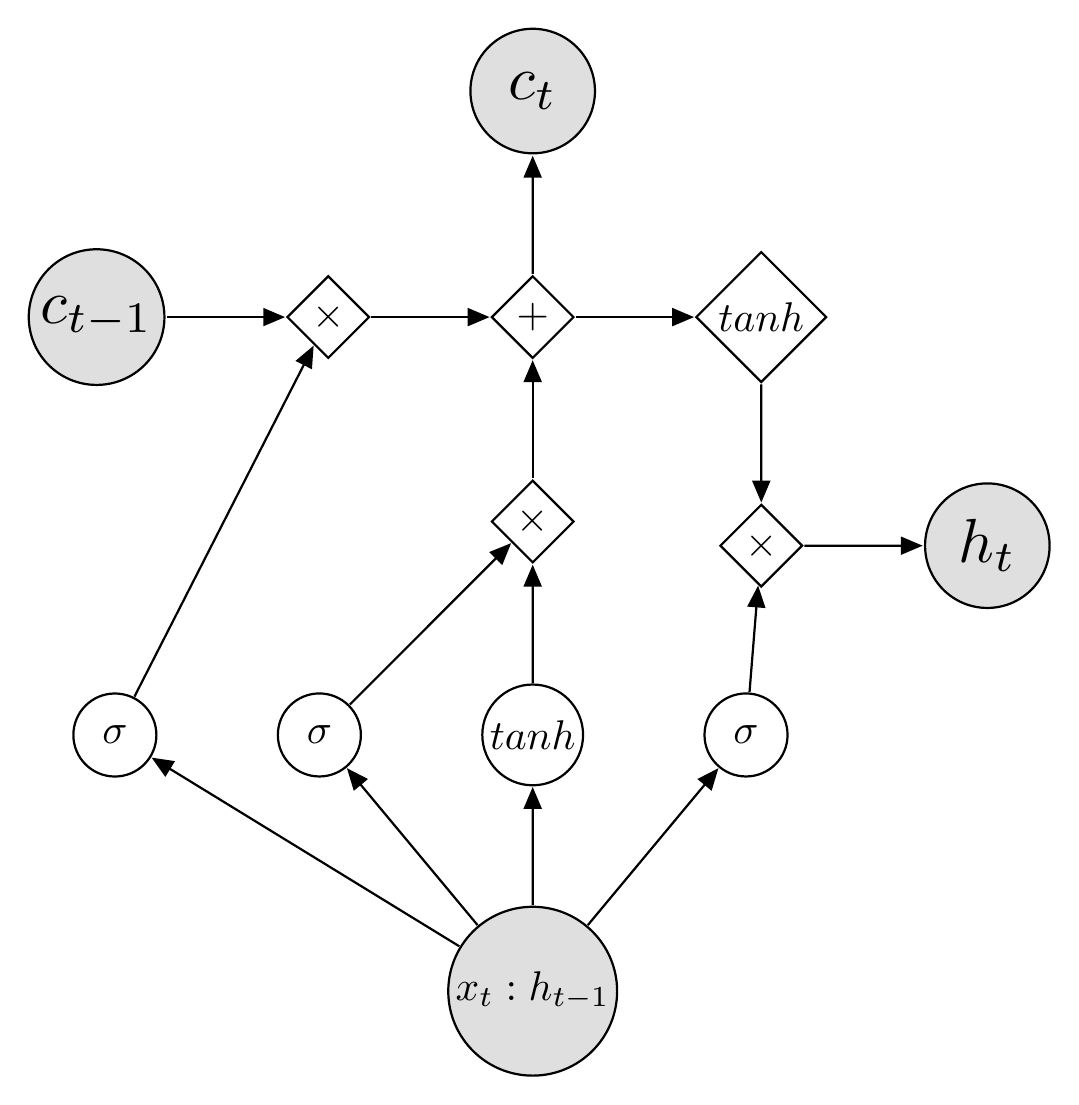
\begin{tikzpicture}[thick,scale=1.5, every node/.style={transform shape}]
    % Nodes
    \node[det] (inputplus) {$+$};
    \node[det, below = of inputplus] (inputtimes) {$\times$};
    \node[latent, below = of inputtimes] (inputtanh) {$tanh$};
    \node[latent, left = of inputtanh] (inputsig) {$\sigma$};
    \node[latent, left = of inputsig] (forgetsig) {$\sigma$};
    \node[det, above = of forgetsig, left = of inputplus] (forgettimes) {$\times$};
    \node[latent, right = of inputtanh] (outputsig) {$\sigma$};
    \node[det, right = of inputplus] (outputtanh) {$tanh$};
    \node[det, below = of outputtanh] (outputtimes) {$\times$};
    \node[obs, below = of inputtanh] (x) {$x_t : h_{t-1}$};
    \node[obs, right = of outputtimes, scale = 1.5] (h) {$h_t$};
    \node[obs, left = of forgettimes, scale = 1.5] (c) {$c_{t-1}$};
    \node[obs, above = of inputplus, scale = 1.5] (cnext) {$c_{t}$};
    % Connections
    \edge {forgetsig} {forgettimes};
    \edge {forgettimes} {inputplus};
    \edge {inputsig} {inputtimes};
    \edge {inputtanh} {inputtimes};
    \edge {inputtimes} {inputplus};
    \edge {outputtanh} {outputtimes};
    \edge {outputsig} {outputtimes};
    \edge {inputplus} {outputtanh};
    \edge {x} {inputsig};
    \edge {x} {forgetsig};
    \edge {x} {inputtanh};
    \edge {x} {outputsig};
    \edge {outputtimes} {h};
    \edge {c} {forgettimes};
    \edge {inputplus} {cnext};
  \end{tikzpicture}
\end{center}

This cell represents a single layer LSTM model, where the white circles are neural network layers with an activation function, the diamonds are pointwise operations and the dark circles input/output states. This could be used as the full model, in which case the $h_t$ would be the outputs $y_t$ of the system. Alternatively these LSTM cells could be stacked, creating a deep learning model where the $h_{it}$ of each layer $i$ would be the input to the layer $i+1$, where $h_{1t}$ are the original inputs $v_t$.

All this serves to create a model where information can be remembered and forgotten dynamically based on where we are in the input sequence. This is very useful for the purposes of this project as repeated musical phrases and structures could be implicitly captured by the model, as shown to be possible by \cite{eck2008learning}.

LSTMs are currently the cutting edge for many different areas of natural language processing, including language modelling \cite{sundermeyer2012lstm} \cite{pichotta2016using}, speech recognition \cite{han2017ese} and language generation in spoken dialogue systems \cite{wen2016multi}.

For an in-depth discussion on LSTMs, \cite{olah_2015} or \cite{greff2016lstm} is recommended.

\section{Review of Previous Work on Automatic Harmonic Analysis}

A brief review of previous work on chord progression estimation and related works will be presented in this section. Note that this is largely unchanged from the report presented last year.

The field of automatic harmonic analysis of music has seen a wide range of research in the past few decades. Much of this stems from the interpretation of music as a form of language, or at least recognising the similarities between music and natural language and exploiting them to achieve certain tasks. The works of \cite{winograd1968linguistics} and \cite{forte1967syntax} were some of the first applications of computational linguistic theory to the field of music, inspired by the pioneering work of Noam Chomsky on the formal definitions of languages and syntax \cite{lees1957syntactic}. In \cite{winograd1968linguistics} a generative grammar for the parsing of a harmonic phrase was proposed, using an adaptation of the formalism of tonal harmony proposed by \cite{forte1962tonal}. This mechanism was capable of automatically parsing chorales.

An alternative method of harmonic analysis, introduced by \cite{schenker1979harmony}, was used in another computationally assisted, automatic parsing of music in \cite{smoliar1979computer}. Similar to the above, Smolier applied existing NLP parsing techniques to a grammatical formalism of tonal music.

Logic based approaches have also been attempted. In \cite{ebciouglu1990expert} an expert system for the harmonic analysis of chorales is proposed, based on first order predicate logic. This was expanded on by \cite{maxwell1992expert}, where a full approach applicable to all tonal music was presented. A similar hierarchical logical representation for the computational analysis of music was proposed by \cite{smaill1993hierarchical}.

The development of probabilistic machine learning algorithms allowed for a more statistical approach to harmonic analysis to be developed. The work of \cite{laden1989representation} applies neural networks to chord classification, focusing on the problem of how to best represent pitch. A more qualitative perception model for musical learning is presented in \cite{widmer1992qualitative}.

A popular and successful method of probabilistic harmonic analysis is the HMM based approach. The harmonic analysis of chorales proposed in \cite{allan2005harmonising} uses HMM probabilistic inference. In \cite{lee2004ring} an HMM based method for chord generation from a hummed input is presented. A simple frequency count based HMM is used in the chordal analysis of the MySong application by Microsoft \cite[]{mysong}, a system that automatically generates an accompaniment for a real-time vocal input. A more complex HMM based system is utilised by \cite{ryynanen2008automatic} in the automatic transcription of melody and chords from the first eight Beatles albums.

The HMM based approach shall form the basis of the baseline model for this project, where in the following year the markov assumption shall be replaced with a more complex grammar based language model. 

In more recent years, a template based approach to chordal analysis has been proposed, notably in the work of \cite{pardo2002algorithms}, \cite{oudre2009template} and \cite{oudre2011probabilistic}. This method moves away from more statistical techniques and instead assigns a rule-based scoring to a frame, based on whether the observed notes are present in the stored chord model template.

More complex hybrid approaches have also been attempted. A combination of neo-Riemannian transformations, Markov chains and Support Vector Machines are used in \cite{chuan2007hybrid} for the generation of style-specific accompaniment. This method uses machine learning techniques to decide how probable it is that an observed note is a 'chord tone' for the current chord and is the inspiration for one of the proposed emission models in this report.  

It should be noted that the majority of these approaches assume pre-segmentation of the input into distinct chord segments for classification, as does the work presented in this report. A complete model of chordal analysis must take this aspect into account as well. There are many well researched methods for accomplishing this, a good review of a few of these is provided in \cite{pardo2002algorithms}.

%Specify everything I did and why!!!
\chapter{Design and Implementation}
The aim of this chapter is to take the reader through the design of the models, by way of example on a piece from the KP Corpus, and to explain the details of the implementation. The models based on HMMs differ in structure from the LSTM models so they is a section for each of these.

\section{Hidden Markov Model Based System}
\subsection{Design} \label{HMM DES}

The first year of this project was focussed on building a HMM based approach to the problem of chord labelling, with a view to use it as comparison to a model that was able to capture a higher level of structure this year. This section will briefly discuss the design of the HMM system, with a focus on a new design that was implemented this year, see \cite{self} for an in depth description of the previous year's implementations.

MINUET IN G

Above is the example piece from the previous chapter, Minuet in G (often attributed to Bach). To reiterate, the task is to take as input the sequence of notes in both staves and to predict the sequence of chord labels. The first thing to notice is that there is not a one-to-one mapping between notes and chord label, there are many more of the former. If we let the chord labels be the latent variables $\{h_t\}_{t=1}{T}$ of our HMM and the notes be $\{v_t\}_{t=1}{T}$, then $v_t$ represents a group of notes that is generated by one chord. This concurs with our intuition of the problem, where in essence we are using the HMM to model the `generation' of notes by a sequence of chords. We can think of this as a song generating machine that can be in a number of states, each state representing a chord. This starts in some state and outputs of group of notes, then transitions to another state and outputs a new sequence of notes. In our example the first state would be the chord of $G$, and the first group would be the first two bars of notes, where the second state is the chord $C$ and the second group is just the third bar of notes.

The models of the first year of this project used exactly this assumption and addressed the problem of going from a sequence of note groups to a sequence of chords. The inherent difficulties in this are that, for each state in the HMM, a smaller model must be constructed to capture the generation of this note group. Three approaches were used, one being a smaller HMM for each step, one being a `bag of notes' model, analogous to a `bag of words' model in natural language processing \cite{bag of words}, and another more complex decision tree model. However these models do not capture how to split the observed notes into groups to start off with, so some pre-processing was assumed and necessary in the experiments. This is unsatisfactory as it does not provide a full model of the problem. Another, more fundamental problem is that the above assumptions discard a crucial indicator of the chord transitions. That is, the transitions between the notes at the end of one group and the beginning of the other. In the example, on the transition from the second chord $C$ to the third chord, another $G$, there is a transition from an $F\#$ note to a $G$ note one semitone above it. This is a key indicator of a chord transition as it the melody is stepping up to the root note of the chord from the note below. This is something that would be beneficial to capture in the model.

Hence a new design of the HMM system is proposed and implemented this year, before the step to LSTMs. Consider a modification to the above machine. This machine outputs a sequence of notes one at a time, starting in some state. The time steps now correspond to each note, not to each chord, hence the machine is essentially self-transitioning for each note in the chord group. Then at some point the machine will transition to a new state and start generating more notes, but from this new state. The task is now to take the full sequence of notes and to try to determine to most likely sequence of states this machine was in when it generated them. Note that we now have a one-to-one mapping between the sequence of notes and the sequence of chords, see the re-labelling of the example below:

RELABEL MINUET IN G

This corresponds to the following HMM:

HMM Graph

Now the $v_t$ each correspond to a single note, and the probabilistic model of $P(v_t | h_t)$ is a simple multinomial distribution that can be observed from the training data, instead of a complex mini-sequence generation task.

Below an sample of the results of the HMM model will be analysed for our example excerpt to shed light on what this model can and can't capture.

DIAGRAM OF RESULTS OF RUNNING HMM ON MINUET IN G

PROBLEM - GUESSED ALL TONIC - REWRITE BELOW

STILL INCLUDE BELOW BUT ALSO EVALUATE OTHER SONG

The first thing to note is that, as discussed later, each song is transposed to the same key to improve training. The above results are not from that model, they are from a model trained with un-transposed songs. This is because, for this particular song and some others, the HMM determines that:

\begin{itemize}
  \item The majority of notes observed will occur when the tonic chord is played
  \item The majority of chords played are the tonic
\end{itemize}

Hence the model guessed the tonic chord for every single position. This is an enlightening problem with the HMM model.

\subsection{Implementation} \label{HMM IMP}

To implement the Hidden Markov Model used in the previous year's work, it was necessary to be modular in approach, with a re-usable high level structure of state transitions (the Transition Model) and a pluggable variety of chord state to note group models (the Emission Model). This allowed for the implementation and testing of the three main emission models described above. However, the majority of HMM libraries that exist in Python, the chosen language for this project, are restricted to basic Gaussian and Multinomial emission models \cite{lebedev_2015} \cite{buitinck}. For this reason the decision was made to implement or more general HMM class that could be modified for each case of emission model. This involved implementing the Viterbi Algorithm \cite{forney1973viterbi}, a dynamic programming method of the determining the most likely sequence of hidden states in a HMM.

Note that this implementation HMMs was purely for supervised learning, where the hidden states are known in the training data. This is fine for the high level structure where HMMs are used to predict chords, but for one of the emission models HMMs were used for the note groups at a lower level as well, where the hidden states are not as clear. In the previous year a second level of labels was added for this purpose, based on a system that measured likely the note was to appear in a version of the chord (c.f. chord tones). For this year of the project one new implementation that was added was an unsupervised HMM that could approximate these hidden states on its own, using the expectation maximisation (EM) algorithm \cite{moon1996expectation}. As this was only required for lower level use, with a multinomial emission, the {\tt hmmlearn} \cite{lebedev_2015} Python library was used.

The major alteration to the HMM model, discussed in the previous section, also had a relatively simpler emission model, compared to the previous year, and so the {\tt seqlearn} Python library \cite{buitinck} was also made use of, for the supervised training of the model, allowing the system to benefit from optimisation that was not possible in the previous implementation of supervised HMMs.

For this new supervised HMM it was also necessary to replicate the observed chord labels for each note in the data. One small design decision that was necessary was the case of polyphonic melodies, where more than one note is played at once. For this case it was sufficient to treat these notes as being played after each other in quick succession, with order being split arbitrarily. In this sense the chords in the melodies are being split into arpeggios.

One key problem in the implementation of these systems is how to model sequential data. Mutable list structures in Python are inefficient at storing large quantities of data. Internally they are actually stored as arrays, not linked lists \cite{rockyb_2015}, so lookup for individual values are still $O(1)$, but Python lists are actually an array of pointers to Python objects. Numpy arrays \cite{numpy_2005} however are highly optimised, storing arrays of uniform type values, requiring a lot less space. But importantly for sequences of undetermined size, a Python list will require $O(k)$ time complexity if the lists size goes beyond the pre-defined allocated memory. This not an ideal method of dealing with sequential data, where we have high dimensions of data of undefined size.

One method for dealing with this problem is to concatenate the sequences into a single dimension and to store this as a Numpy array. For this implementation each note is stored as size 12 one-hot vector, where each index corresponds to a note pitch and the vector contains zeros at every index except that corresponding to the note it encodes. In this way we are treating notes as categorical data, avoiding the inherent ordering of storing them as integers. Hence we can store all the data as a 2 dimensional, $D \times T$, Numpy array, where $D$ is the number of notes (12) and:

\begin{align}
  T = \sum_{i=1}^{N} t_i
\end{align}

where $N$ is the number of songs and $t_i$ is the number of notes in song $i$. So the sequences of notes in each song have been concatenated together into a single data structure. A similar operation is done for the chord labels, of which there are also 12 as, for the purposes of experiments, only the roots of the chords are chosen as the labels, see section \ref{preprocessing}.

Another benefit of storing data as Numpy arrays is the benefit of optimised matrix operations, in contrast to index iteration for the implementation of certain algorithms. This doesn't affect the HMM model but is very important when using neural networks see section \ref{LSTM IMP}

\section{Recurrent Neural Network Based System}
We now move on to the LSTM based system and the design decisions that were involved in building it. 

\subsection{Design}
The HMM is a very good approximate model with an intuitive understanding but it's main drawback is the first order markov assumption. We know from music theory that the is an underlying structure in the design of chord progressions \cite{krumhansl1982perceived} \cite{piston1948harmony}. One possible approach for making use of this structure would be to incorporate a grammatical `language' mode of chord progressions, as constructed by \cite{granroth2014robust} or \cite{rohrmeier2007generative}. The approach taken in this project was to instead build a system that could learn to an implicit representation of structure with memory. This was inspired by the success of such systems at learning language models in other applications, see \cite{schmidhuber2002learning} \cite{sundermeyer2012lstm}. Hence the decision was made to build an LSTM based sequence to sequence model.

In general a sequence to sequence model refers to the combination of an encoder and a decoder, taking an input sequence to and output sequence, each of which can have a different length. This would have been possible to implement for this problem, but due to the direct local relationship of chords to notes it was decided that a simpler system would be more beneficial. This design makes use of the repeated representation of the data, where there is a one-to-one mapping between chord labels and notes. We can then use a model where each LSTM cell's output is treated as a chord in the prediction sequence. Graphically (and abstractly for simplification) we are modifying the model to take this structure:

LSTM GRAPHICAL MODEL (add cell state to HMM model)

Instead of only passing the information of which chord was last played to the next state, this model allows for the passing of abstract learned information from time $t-1$ to time $t$. This allows the system to model a more complex, context-dependent relationship between the current note and the current chord. For example the note $E$ on its own is not very likely to be played over a $D major$ (the triad notes of a $D major$ are $D$, $F\#$ and $A$, an E would be dissonant), but if it's preceded by a $D$ then it could be an intermediate note between $D$ and $F\#$. This relationship can be implicitly captured by the Viterbi algorithm for HMMs in the prediction of the most likely sequence (the chord sequence is not likely to jump to an $E major$ for a single note then back again) but in this way this information can be directly encoded in the LSTM model. Something that an HMM might not be able to capture is that if, say, the chord progression $G major$, $G\# diminished$, $A minor$ occurred at one point in the song, then if $G major$, $G\# diminished$ at some point later then a very probable next chord is the same $A minor$. Concepts like repeated structure (at note level too) and long term dependencies are theoretically able to be captured by the LSTM. In practice it is very difficult to determine whether this is has happened, as the information is encoded in the weight matrices of the LSTM cell, not an easily readable probability table.

ANALYSIS OF MINUET IN G

\subsection{Implementation} \label{LSTM IMP}

In recent years new, open source tools have been made available to facilitate the implementation of machine learning (ML) algorithms. One notable example is Tensorflow \cite{tensorflow2015-whitepaper}, a highly optimised platform for creating ML architectures as a computation graph in C++, with a Python interface. Tensorflow has a symbolic, declarative structure. Variables and interactions between them such as matrix multiplications (a key operation in neural networks) are defined fully before any computation on data occurs, then a session is opened and the data is passed through the computation graph. This has proven to be a very powerful tool and it is now widely used in the field.

A higher level, specifically neural network aimed Python API exists, built on a Tensorflow backend, called Keras \cite{chollet2015}. This framework abstracts away low level implementation of weight matrices and gradient calculation to allow design at the level of neural network layers and declarative algorithm choices. This library has proved very useful for research as it allows for quick, reliable design and experimentation on neural networks. These two libraries, Keras with a Tensorflow backend, were used in the implementation of the LSTM model.

After general preprocessing (see the next section), it was necessary to transform the data into a form that could be processed by the LSTM model. This is the same problem of modelling sequential data face by the HMM. An alternate solution was used on this model, one in-line with the guidelines of the libraries used. Instead of concatenating the data into one dimension, it more beneficial for a system based on matrix multiplication, such as neural networks, to have more smaller dimensions, over-which these operations can efficiently be performed. Accordingly, our previously 2-dimensional data (pitch $\times$ full note sequence) is now modelled as a 3-dimensional tensor (pitch $\times$ song note sequence $\times$ songs). However this now poses a problem: The pitch dimension is always size 12 but there are a varying number of notes in each song. The solution is to simply pad the ends of each song with a special $PAD$ vector so that every song is the length of the longest song, which will have no padding, where the $PAD$ vector is implemented as the zero vector. This raises problems of its own, such as efficiency of checking the maximum length, and transferability to an on-line setting (how can you know if a longer song might appear next?), but it is suitable to the purposes of this project.

This padded data is then fed into the first layer of the model, which is a masking layer that looks for the padding and masks it from influencing the rest of the layers while maintaining dimension size. This is, helpfully, a provided feature of Keras. The next step is the main LSTM layer, implemented with dropout to avoid overfitting on the training data, the hyper-parameters of which experiments were run over. Each LSTM cell in this layer outputs a vector which is then fed into a time distributed fully connected layer with softmax activation. Essentially this is a standard, dense neural network layer that takes the outputted vector of the LSTM cell to a $K$ dimensional vector of probabilities over each chord, where $K$ is the number of chords (typically 12 in this study). This dense layer is then repeated for every time step in the sequence, as the LSTM cell is a layer below. These softmax output logits are then used to predict the most likely chord, akin to the multinomial output of the HMM.

LSTM KERAS DIAGRAM

The model described above is the most simple of those used, for experiments on more complex structures see chapter \ref{Experimental Results}.

The next step is to train the model. The loss function used for this training was the categorical cross-entropy between the logits and the true labels \cite{shore1980axiomatic}. This is a method for measuring the `distance' between two probability distributions (the labels can be considered a probability distribution with certainty on the true value) and can be defined as follows:

\begin{align}
  E(\bm{y}, \bm{t}) = - \sum_{i=1}^{T}\sum_{k=1}^{K} t_{i_k} \mathrm{log}(y_{i_k})
\end{align}

The gradient descent algorithm used for training was Root Mean Square Propagation (RMSProp), an idea proposed by Hinton and Tieleman in 2012 \cite{tieleman2012lecture}. The idea here is to, for each weight, divide the learning rate by a factor proportional to a running average of the size of that weight's gradient:

\begin{align}
  w_{i_j}^{(t+1)} = w_{i_j}^{(t)} - \frac{\eta}{v(w_{i_j}, t)} \frac{\partial E(\bm{y}, \bm{t})}{\partial w_{i_j}}
\end{align}

where $v(w_{i_j}, t)$ is the running average of the gradient size (implemented with a forget parameter) and $\eta$ is the learning rate. Note that in the model there are more than just two indices needed to identify all the weights, $i$ and $j$ here are used to simplify illustration.

Another small consideration that was needed was to carefully weight the cross entropy loss to avoid taking the padding into account. Astonishingly high faux-accuracies and over-early celebrations were almost avoided.

One advantage of the Tensorflow backend is that it is highly optimised to GPUs. The more complex models with more weights were trained on the university's compute {\tt msccluster} which has access to 3 Geforce Titan X Nvidia GPUs in each node.

\section{Preprocessing} \label{preprocessing}

This section briefly details the general pre-processing that was necessary for converting the data from its raw state to a form that could be processed by the models. The datasets used for the experiments are described in detail in section \ref{Datasets} but each provides data in very different forms, so each will be broken down here.

\subsection{Weimar Jazz Database}

The Weimar Jazz Database (see \ref{wjazz}) provides a graphical user interface packaged with pre-processing tools for the extraction of features from its dataset. The data used for this project in the first year made use of many of these features (metrical information etc.) but the models of this year abstract the melody as a simple sequence of 12 possible pitch classes (i.e. C through B$\flat$). Hence the data was exported as a {\tt csv} file of pitch classes with matching chord labels as strings. Note that these pitch classes are transposed to the same key, hence a 0 in the key of $C$ will be a $C$ note, but a 0 in the key of $G$ will be a $G$ note. These pitch classes are hence called Tonal Pitch Classes (TPCs).

The transposition of all songs to the same key (the key of $C$) is beneficial to the design of all models as it allows for relative relationships to be learned, not just absolute relationships. Hence this is included in the design of the system, although it should be noted that in some cases the models make `more interesting' mistakes without transposition, see the results section.

The chord strings are then converted pitch classes, and then transposed to TPCs, to be used as chord labels. All TPCs were then converted into one hot vectors. The reading of the {\tt csv} files, preprocessing and the collation into arrays for further processing is packaged into a {\tt DataLoader} class.

\subsection{KP Corpus}

The data from the KP Corpus (see \ref{kp}) is provided in Musical Instrument Digital Interface (MIDI) format. MIDI files consist of {\tt note\_on} and {\tt note\_off} events of varying length and pitch, arranged into a list, plus some meta data. The chord labels for this corpus are provided as annotated lyrics in the MIDI files.

The {\tt midicsv} \cite{walker_2008} utility was used to convert the MIDI files to {\tt csv} format, with no other processing, allowing the {\tt note\_on} and {\tt note\_off} events to be read into Python. More complex preprocessing was then required to generate a sequence of TPCs, implemented in a separate {\tt DataLoader} class for this dataset. Transposition and chord label extraction was done in a similar way to the previous Weimar Jazz Database.

%Detail every single run of things, talk about data things
\chapter{Experimental Results} \label{Experimental Results}

In this chapter the datasets used, experimental design and main results of the project will be presented and discussed.

\section{Datasets} \label{Datasets}
A key problem with analysing the harmonic structure of melodies is the availability of data. Primarily due to copyright issues, much of the data used by similar projects in the literature is not made available publicly. What is available is largely just melodic, without chord annotations \cite{turetsky2003ground} \cite{MuellerKBA11_SMD_ISMIR-lateBreaking}. Some purely harmonic datasets also exist \cite{burgoyne2011expert} \cite{digiorgi2013automatic}, but this task requires the aligning of the two for training and analysis.

\subsection{Weimar Jazz Database} \label{wjazz}
The dataset used for the previous year's work was the Weimar Jazz Database \cite{wjazz}. This is a collection of 273 transcribed solos from famous Jazz musicians, typically over a Jazz Standard (a commonly known piece of jazz music over which a group of musicians will improvise). The meta data in this data set is extensive and of a very high quality, but inherent difficulties come in domain of melodies. Improvised jazz solos are, in a music theoretic sense, very noisy. They tend to be unpredictable and ambiguous harmonically, increasing the difficulty of this problem.

EXAMPLE

\subsection{KP Corpus} \label{kp}
The first main task of this year's work was to find a new database that contained simpler melodies, on which the models of last year could be retrained on and on which the new models could be developed. For the reasons stated above this was a difficult search. The dataset the was settled on was a collection of excerpts from classical songs in MIDI format. These melodies are much simpler and easier to analyse, with a stronger correlation between notes and chords. The example used earlier, Minuet in G (shown below) is from this dataset. The only downside of this corpus is that there are only 46 excerpts, a small number for training and evaluating stochastic models.

MINUET IN G

\section{Accuracy Metric}



\section{Baselines}

\section{HMM Results}

\section{LSTM Results} \label{LSTM Results}

\section{Other Results}


\chapter{Conclusion}

\section{Discussion}

\section{Future Work}

% use the following and \cite{} as above if you use BibTeX
% otherwise generate bibtem entries
\bibliographystyle{acm}
\bibliography{bibfile}

\end{document}
